\documentclass[residuals.tex]{subfiles}
\Large
\begin{document}
\newpage
\Large
\section{Some Important Definitions}

%\newpage
%\subsection{More Definitions}
To understand a diagnostic plot called the residual-leverage plot, we must understand three things:

\begin{itemize}
	\item Leverage,
	\item Standardized residuals, and
	\item Cook's distance.
\end{itemize}
%Move next bit to "Leverarge"

% Standardization

% Cook's Distance
%\subsubsection{Cook's Distance}
%One way to think about whether or not the results you have were driven by a given data point is to calculate how far the predicted values for your data would move if your model were fit without the data point in question. 

%This calculated total distance is called \textbf{Cook's distance}. Fortunately, you don't have to rerun your regression model N times to find out how far the predicted values will move, Cook's D is a function of the leverage and standardized residual associated with each data point.

\subsection*{Example}

Consider the plots associated with four different situations:
\begin{enumerate}
	\item a dataset where everything is fine
	\item a dataset with a high-leverage, but low-standardized residual point
	\item a dataset with a low-leverage, but high-standardized residual point
	\item a dataset with a high-leverage, high-standardized residual point
\end{enumerate}
\newpage
\begin{figure}[h!]
	\centering
	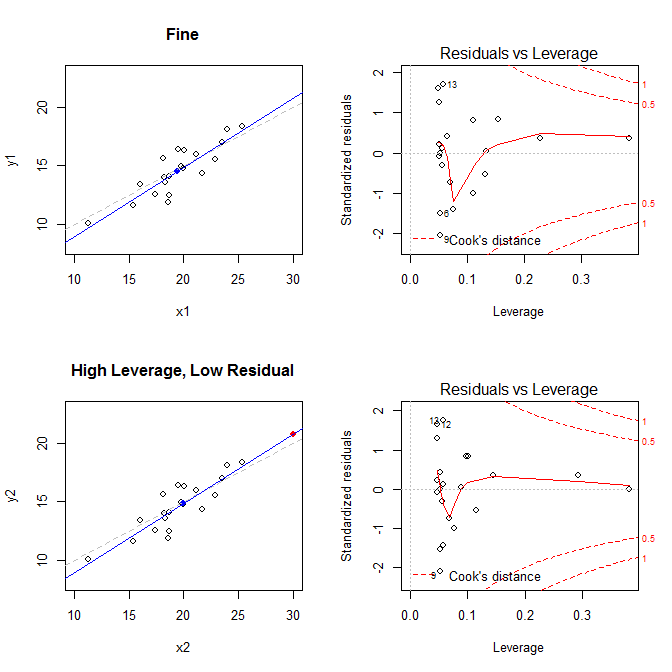
\includegraphics[width=1.0\linewidth]{plots2}
	\caption{}
	\label{fig:plots2}
\end{figure}
\newpage
\begin{figure}[h!]
\centering
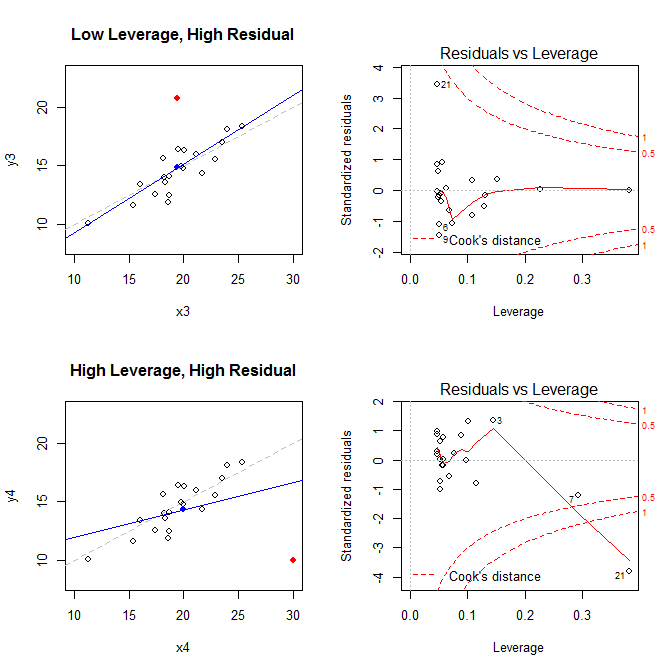
\includegraphics[width=1.0\linewidth]{plots3}
\caption{}
\label{fig:plots3}
\end{figure}
\newpage
\begin{itemize}
\item The plots on the left show the data, the center of the data  with a blue dot, the underlying data generating process with a dashed gray line, the model fit with a blue line, and the special point with a red dot. 
\item On the right are the corresponding residual-leverage plots; the special point is 21. 
\item The model is badly distorted primarily in the fourth case where there is a point with high leverage and a large (negative) standardized residual. 

\end{itemize}

For reference, here are the values associated with the special points:
\begin{verbatim}
                               leverage std.residual   cooks.d
high leverage,  low residual  0.3814234    0.0014559 0.0000007
low leverage,  high residual  0.0476191    3.4456341 0.2968102
high leverage, high residual  0.3814234   -3.8086475 4.4722437
\end{verbatim}
\end{document}
